\documentclass[twoside]{book}

% Packages required by doxygen
\usepackage{calc}
\usepackage{doxygen}
\usepackage{graphicx}
\usepackage[utf8]{inputenc}
\usepackage{makeidx}
\usepackage{multicol}
\usepackage{multirow}
\usepackage{textcomp}
\usepackage[table]{xcolor}

% Font selection
\usepackage[T1]{fontenc}
\usepackage{mathptmx}
\usepackage[scaled=.90]{helvet}
\usepackage{courier}
\usepackage{amssymb}
\usepackage{sectsty}
\renewcommand{\familydefault}{\sfdefault}
\allsectionsfont{%
  \fontseries{bc}\selectfont%
  \color{darkgray}%
}
\renewcommand{\DoxyLabelFont}{%
  \fontseries{bc}\selectfont%
  \color{darkgray}%
}

% Page & text layout
\usepackage{geometry}
\geometry{%
  a4paper,%
  top=2.5cm,%
  bottom=2.5cm,%
  left=2.5cm,%
  right=2.5cm%
}
\tolerance=750
\hfuzz=15pt
\hbadness=750
\setlength{\emergencystretch}{15pt}
\setlength{\parindent}{0cm}
\setlength{\parskip}{0.2cm}
\makeatletter
\renewcommand{\paragraph}{%
  \@startsection{paragraph}{4}{0ex}{-1.0ex}{1.0ex}{%
    \normalfont\normalsize\bfseries\SS@parafont%
  }%
}
\renewcommand{\subparagraph}{%
  \@startsection{subparagraph}{5}{0ex}{-1.0ex}{1.0ex}{%
    \normalfont\normalsize\bfseries\SS@subparafont%
  }%
}
\makeatother

% Headers & footers
\usepackage{fancyhdr}
\pagestyle{fancyplain}
\fancyhead[LE]{\fancyplain{}{\bfseries\thepage}}
\fancyhead[CE]{\fancyplain{}{}}
\fancyhead[RE]{\fancyplain{}{\bfseries\leftmark}}
\fancyhead[LO]{\fancyplain{}{\bfseries\rightmark}}
\fancyhead[CO]{\fancyplain{}{}}
\fancyhead[RO]{\fancyplain{}{\bfseries\thepage}}
\fancyfoot[LE]{\fancyplain{}{}}
\fancyfoot[CE]{\fancyplain{}{}}
\fancyfoot[RE]{\fancyplain{}{\bfseries\scriptsize Generated on Sat Nov 2 2013 16:14:46 for DataStructures4Beamer by Doxygen }}
\fancyfoot[LO]{\fancyplain{}{\bfseries\scriptsize Generated on Sat Nov 2 2013 16:14:46 for DataStructures4Beamer by Doxygen }}
\fancyfoot[CO]{\fancyplain{}{}}
\fancyfoot[RO]{\fancyplain{}{}}
\renewcommand{\footrulewidth}{0.4pt}
\renewcommand{\chaptermark}[1]{%
  \markboth{#1}{}%
}
\renewcommand{\sectionmark}[1]{%
  \markright{\thesection\ #1}%
}

% Indices & bibliography
\usepackage{natbib}
\usepackage[titles]{tocloft}
\setcounter{tocdepth}{3}
\setcounter{secnumdepth}{5}
\makeindex

% Hyperlinks (required, but should be loaded last)
\usepackage{ifpdf}
\ifpdf
  \usepackage[pdftex,pagebackref=true]{hyperref}
\else
  \usepackage[ps2pdf,pagebackref=true]{hyperref}
\fi
\hypersetup{%
  colorlinks=true,%
  linkcolor=blue,%
  citecolor=blue,%
  unicode%
}

% Custom commands
\newcommand{\clearemptydoublepage}{%
  \newpage{\pagestyle{empty}\cleardoublepage}%
}


%===== C O N T E N T S =====

\begin{document}

% Titlepage & ToC
\hypersetup{pageanchor=false}
\pagenumbering{roman}
\begin{titlepage}
\vspace*{7cm}
\begin{center}%
{\Large Data\-Structures4\-Beamer \\[1ex]\large 1.\-0 }\\
\vspace*{1cm}
{\large Generated by Doxygen 1.8.4}\\
\vspace*{0.5cm}
{\small Sat Nov 2 2013 16:14:46}\\
\end{center}
\end{titlepage}
\clearemptydoublepage
\tableofcontents
\clearemptydoublepage
\pagenumbering{arabic}
\hypersetup{pageanchor=true}

%--- Begin generated contents ---
\chapter{Documentation}
\label{index}\hypertarget{index}{}Data\-Structures4\-Beamer is a library created for any help learning how abstract data structure, the library is basically provide the methods necessary for the developer to create and manage data structures, plus it generates a pdf file based on the structure data that is being used, the file shows each phase the structure is subjected.

Caveats aside, you might get started learning about abstract data structures reading the recommended lectures , those are located in Related Pages.

The library were specifically designed to be used with C++ and Latex, both important dependencies that are necessary for use this library. 
\chapter{Recommended Lectures}
\label{page1}
\hypertarget{page1}{}
\hypertarget{page1_sec0}{}\section{Data Structures}\label{page1_sec0}
\href{http://en.wikipedia.org/wiki/Data_structure}{\tt http\-://en.\-wikipedia.\-org/wiki/\-Data\-\_\-structure} \hypertarget{page1_sec1}{}\section{Graph Theory}\label{page1_sec1}
\href{http://en.wikipedia.org/wiki/Graph_theory}{\tt http\-://en.\-wikipedia.\-org/wiki/\-Graph\-\_\-theory} \hypertarget{page1_subsection1}{}\subsection{Array}\label{page1_subsection1}
\href{http://en.wikipedia.org/wiki/Array}{\tt http\-://en.\-wikipedia.\-org/wiki/\-Array} \hypertarget{page1_subsection2}{}\subsection{Linked List}\label{page1_subsection2}
\href{http://en.wikipedia.org/wiki/Linked_list}{\tt http\-://en.\-wikipedia.\-org/wiki/\-Linked\-\_\-list} \hypertarget{page1_subsection3}{}\subsection{Queue}\label{page1_subsection3}
\href{http://en.wikipedia.org/wiki/Queue_%28abstract_data_type%29}{\tt http\-://en.\-wikipedia.\-org/wiki/\-Queue\-\_\-\%28abstract\-\_\-data\-\_\-type\%29} \hypertarget{page1_subsection4}{}\subsection{Stack}\label{page1_subsection4}
\href{http://en.wikipedia.org/wiki/Stack_%28abstract_data_type%29}{\tt http\-://en.\-wikipedia.\-org/wiki/\-Stack\-\_\-\%28abstract\-\_\-data\-\_\-type\%29} \hypertarget{page1_subsection5}{}\subsection{Binary Tree}\label{page1_subsection5}
\href{http://en.wikipedia.org/wiki/Binary_tree}{\tt http\-://en.\-wikipedia.\-org/wiki/\-Binary\-\_\-tree} 
\chapter{Hierarchical Index}
\section{Class Hierarchy}
This inheritance list is sorted roughly, but not completely, alphabetically\-:\begin{DoxyCompactList}
\item \contentsline{section}{Latex}{\pageref{class_latex}}{}
\begin{DoxyCompactList}
\item \contentsline{section}{Lista}{\pageref{class_lista}}{}
\end{DoxyCompactList}
\item \contentsline{section}{Nodo}{\pageref{class_nodo}}{}
\end{DoxyCompactList}

\chapter{Class Index}
\section{Class List}
Here are the classes, structs, unions and interfaces with brief descriptions\-:\begin{DoxyCompactList}
\item\contentsline{section}{\hyperlink{class_arreglo}{Arreglo} }{\pageref{class_arreglo}}{}
\item\contentsline{section}{\hyperlink{class_latex}{Latex} }{\pageref{class_latex}}{}
\item\contentsline{section}{\hyperlink{class_lista}{Lista} }{\pageref{class_lista}}{}
\item\contentsline{section}{\hyperlink{class_nodo}{Nodo} }{\pageref{class_nodo}}{}
\end{DoxyCompactList}

\chapter{File Index}
\section{File List}
Here is a list of all files with brief descriptions\-:\begin{DoxyCompactList}
\item\contentsline{section}{/home/mtorres/\-Dropbox/\-Universidad/\-Estructuras/\-Proyecto1/\-Fox\-Hound/src/\hyperlink{array_8cpp}{array.\-cpp} }{\pageref{array_8cpp}}{}
\item\contentsline{section}{/home/mtorres/\-Dropbox/\-Universidad/\-Estructuras/\-Proyecto1/\-Fox\-Hound/src/\hyperlink{array_8h}{array.\-h} }{\pageref{array_8h}}{}
\item\contentsline{section}{/home/mtorres/\-Dropbox/\-Universidad/\-Estructuras/\-Proyecto1/\-Fox\-Hound/src/\hyperlink{latex_8cpp}{latex.\-cpp} }{\pageref{latex_8cpp}}{}
\item\contentsline{section}{/home/mtorres/\-Dropbox/\-Universidad/\-Estructuras/\-Proyecto1/\-Fox\-Hound/src/\hyperlink{latex_8h}{latex.\-h} }{\pageref{latex_8h}}{}
\item\contentsline{section}{/home/mtorres/\-Dropbox/\-Universidad/\-Estructuras/\-Proyecto1/\-Fox\-Hound/src/\hyperlink{list_8cpp}{list.\-cpp} }{\pageref{list_8cpp}}{}
\item\contentsline{section}{/home/mtorres/\-Dropbox/\-Universidad/\-Estructuras/\-Proyecto1/\-Fox\-Hound/src/\hyperlink{list_8h}{list.\-h} }{\pageref{list_8h}}{}
\item\contentsline{section}{/home/mtorres/\-Dropbox/\-Universidad/\-Estructuras/\-Proyecto1/\-Fox\-Hound/src/\hyperlink{list__node_8cpp}{list\-\_\-node.\-cpp} }{\pageref{list__node_8cpp}}{}
\item\contentsline{section}{/home/mtorres/\-Dropbox/\-Universidad/\-Estructuras/\-Proyecto1/\-Fox\-Hound/src/\hyperlink{list__node_8h}{list\-\_\-node.\-h} }{\pageref{list__node_8h}}{}
\item\contentsline{section}{/home/mtorres/\-Dropbox/\-Universidad/\-Estructuras/\-Proyecto1/\-Fox\-Hound/src/\hyperlink{main_8cpp}{main.\-cpp} }{\pageref{main_8cpp}}{}
\item\contentsline{section}{/home/mtorres/\-Dropbox/\-Universidad/\-Estructuras/\-Proyecto1/\-Fox\-Hound/src/\hyperlink{test_8cpp}{test.\-cpp} }{\pageref{test_8cpp}}{}
\item\contentsline{section}{/home/mtorres/\-Dropbox/\-Universidad/\-Estructuras/\-Proyecto1/\-Fox\-Hound/src/\hyperlink{to__tex_8cpp}{to\-\_\-tex.\-cpp} }{\pageref{to__tex_8cpp}}{}
\item\contentsline{section}{/home/mtorres/\-Dropbox/\-Universidad/\-Estructuras/\-Proyecto1/\-Fox\-Hound/src/\hyperlink{to__tex_8h}{to\-\_\-tex.\-h} }{\pageref{to__tex_8h}}{}
\item\contentsline{section}{/home/mtorres/\-Dropbox/\-Universidad/\-Estructuras/\-Proyecto1/\-Fox\-Hound/src/\hyperlink{tree_8cpp}{tree.\-cpp} }{\pageref{tree_8cpp}}{}
\item\contentsline{section}{/home/mtorres/\-Dropbox/\-Universidad/\-Estructuras/\-Proyecto1/\-Fox\-Hound/src/\hyperlink{tree_8h}{tree.\-h} }{\pageref{tree_8h}}{}
\item\contentsline{section}{/home/mtorres/\-Dropbox/\-Universidad/\-Estructuras/\-Proyecto1/\-Fox\-Hound/src/\hyperlink{tree__node_8h}{tree\-\_\-node.\-h} }{\pageref{tree__node_8h}}{}
\end{DoxyCompactList}

\chapter{Class Documentation}
\hypertarget{classarray}{\section{array Class Reference}
\label{classarray}\index{array@{array}}
}
Inheritance diagram for array\-:\begin{figure}[H]
\begin{center}
\leavevmode
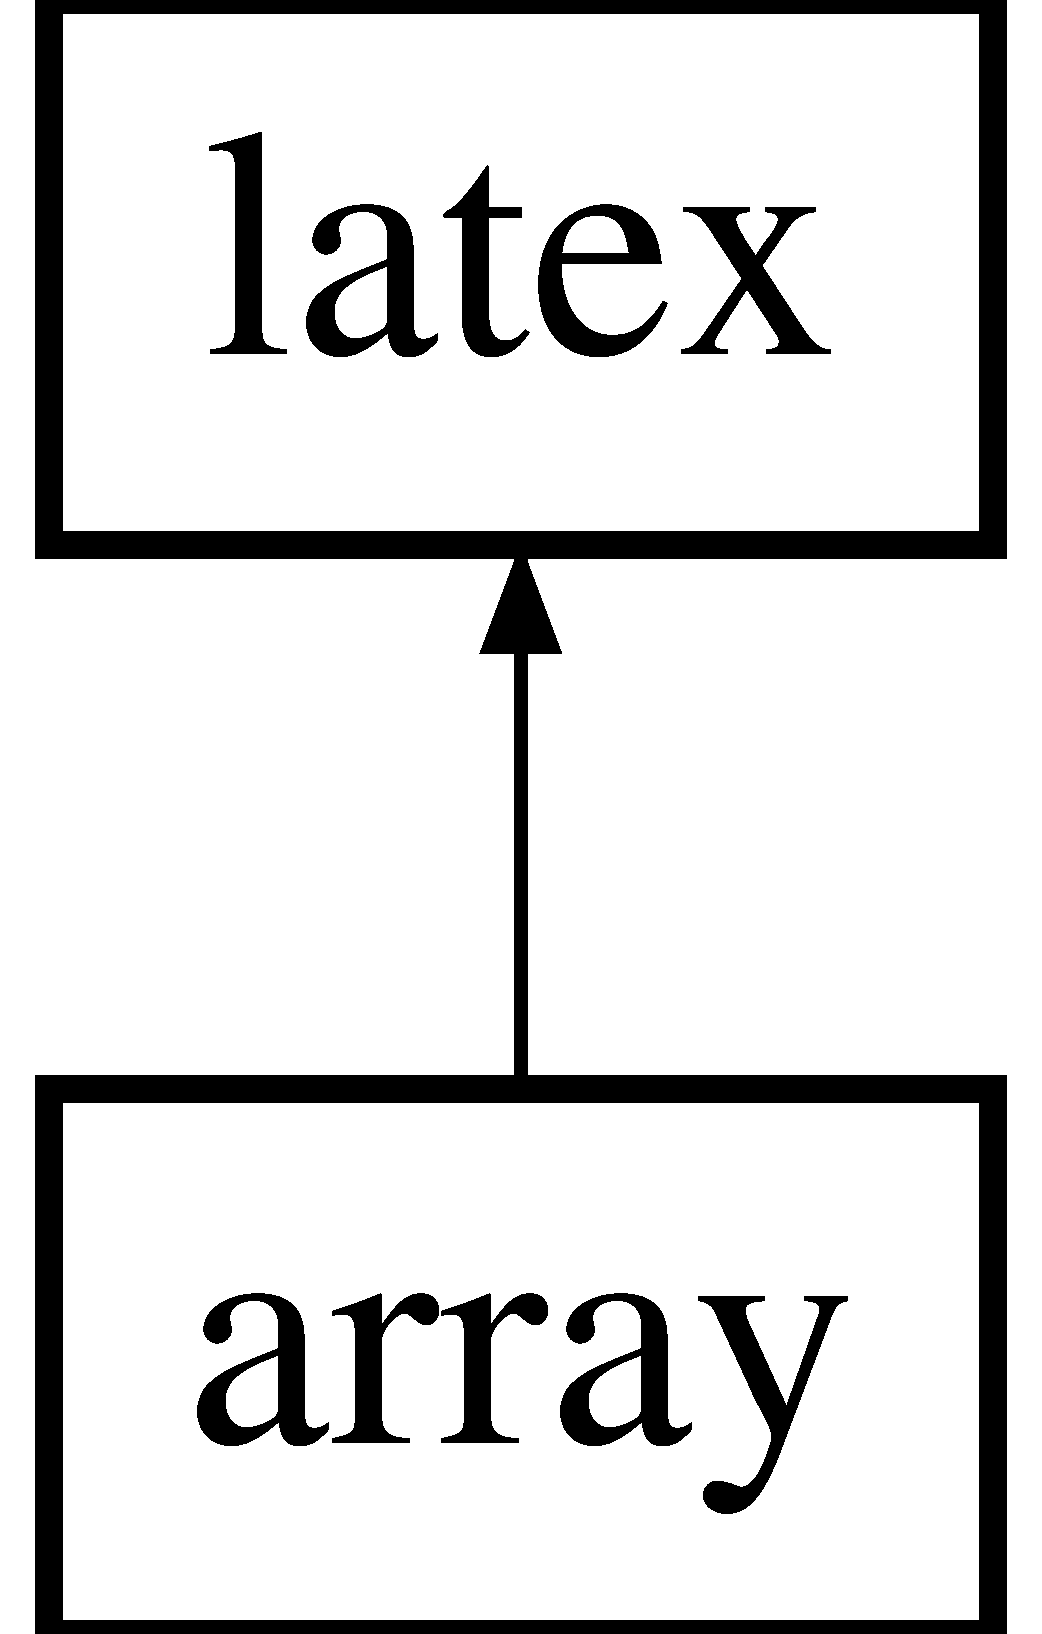
\includegraphics[height=2.000000cm]{classarray}
\end{center}
\end{figure}
\subsection*{Public Member Functions}
\begin{DoxyCompactItemize}
\item 
\hypertarget{classarray_a1264f89751d04076f0c9e40dd548b34a}{int \hyperlink{classarray_a1264f89751d04076f0c9e40dd548b34a}{delete\-\_\-element} ()}\label{classarray_a1264f89751d04076f0c9e40dd548b34a}

\begin{DoxyCompactList}\small\item\em Deletes the first element in the array. \end{DoxyCompactList}\item 
\hypertarget{classarray_a6866ed5e8568471e8fa5012214e8b31b}{void \hyperlink{classarray_a6866ed5e8568471e8fa5012214e8b31b}{delete\-\_\-element\-\_\-in\-\_\-pos} (int)}\label{classarray_a6866ed5e8568471e8fa5012214e8b31b}

\begin{DoxyCompactList}\small\item\em Deletes the element in the position \char`\"{}pos\char`\"{} of the array. \end{DoxyCompactList}\item 
\hypertarget{classarray_aeddcdc0e56dc8cea81f9031200722317}{void \hyperlink{classarray_aeddcdc0e56dc8cea81f9031200722317}{insert\-\_\-element} (int)}\label{classarray_aeddcdc0e56dc8cea81f9031200722317}

\begin{DoxyCompactList}\small\item\em Inserts an element with value \char`\"{}elem\char`\"{} to the first position of the array. \end{DoxyCompactList}\item 
\hypertarget{classarray_a3f88ff1af571a2a320e6ef79de2722fb}{void \hyperlink{classarray_a3f88ff1af571a2a320e6ef79de2722fb}{insert\-\_\-element\-\_\-in\-\_\-pos} (int, int)}\label{classarray_a3f88ff1af571a2a320e6ef79de2722fb}

\begin{DoxyCompactList}\small\item\em Inserts an element with value \char`\"{}elem\char`\"{} to the position \char`\"{}pos\char`\"{} of the array. \end{DoxyCompactList}\item 
\hypertarget{classarray_a1907d4f2b944c0acd6f45d4659e49646}{void \hyperlink{classarray_a1907d4f2b944c0acd6f45d4659e49646}{fill\-\_\-vector} (int)}\label{classarray_a1907d4f2b944c0acd6f45d4659e49646}

\begin{DoxyCompactList}\small\item\em Fills an empty array, assigns zero to each position. \end{DoxyCompactList}\item 
\hypertarget{classarray_aedfc14adc0aaa8398258794564f79b22}{\hyperlink{classarray_aedfc14adc0aaa8398258794564f79b22}{array} (int n=10)}\label{classarray_aedfc14adc0aaa8398258794564f79b22}

\begin{DoxyCompactList}\small\item\em Constructor initializes an array of size \char`\"{}n\char`\"{}. \end{DoxyCompactList}\item 
\hypertarget{classarray_adc0ddb6f7348edf390b97e883f4ee773}{int \hyperlink{classarray_adc0ddb6f7348edf390b97e883f4ee773}{sum\-\_\-vector} ()}\label{classarray_adc0ddb6f7348edf390b97e883f4ee773}

\begin{DoxyCompactList}\small\item\em Returns the sum of all elements in the array. \end{DoxyCompactList}\item 
\hypertarget{classarray_aae5279d424036f187c6aa516bbd83c5c}{int \hyperlink{classarray_aae5279d424036f187c6aa516bbd83c5c}{max} ()}\label{classarray_aae5279d424036f187c6aa516bbd83c5c}

\begin{DoxyCompactList}\small\item\em Returns the element with the highest value in the array. \end{DoxyCompactList}\item 
\hypertarget{classarray_a9787f152f19d3efaa10661fd8ab5d984}{int \hyperlink{classarray_a9787f152f19d3efaa10661fd8ab5d984}{min} ()}\label{classarray_a9787f152f19d3efaa10661fd8ab5d984}

\begin{DoxyCompactList}\small\item\em Returns the element with the lowest value in the array. \end{DoxyCompactList}\item 
\hypertarget{classarray_ac3d618d2d45fc6734b870e69175191a5}{void \hyperlink{classarray_ac3d618d2d45fc6734b870e69175191a5}{invest\-\_\-vector} ()}\label{classarray_ac3d618d2d45fc6734b870e69175191a5}

\begin{DoxyCompactList}\small\item\em Reverses the positions of the elements ​​in the array. \end{DoxyCompactList}\item 
\hypertarget{classarray_a38eae774a7eba29581bf399f33309ffc}{void \hyperlink{classarray_a38eae774a7eba29581bf399f33309ffc}{exchange\-\_\-elements2} (int, int)}\label{classarray_a38eae774a7eba29581bf399f33309ffc}

\begin{DoxyCompactList}\small\item\em Change the position of two elements. \end{DoxyCompactList}\item 
\hypertarget{classarray_a6fc40f0a530525bb91835af4dcd20565}{void \hyperlink{classarray_a6fc40f0a530525bb91835af4dcd20565}{print\-\_\-vector} ()}\label{classarray_a6fc40f0a530525bb91835af4dcd20565}

\begin{DoxyCompactList}\small\item\em Displays the array values right through console. \end{DoxyCompactList}\item 
\hypertarget{classarray_a1e2e2da0c5c43d2a2c6f932036868d38}{int \hyperlink{classarray_a1e2e2da0c5c43d2a2c6f932036868d38}{get\-\_\-amount} ()}\label{classarray_a1e2e2da0c5c43d2a2c6f932036868d38}

\begin{DoxyCompactList}\small\item\em Returns current number of elements contained in the array. \end{DoxyCompactList}\item 
\hypertarget{classarray_a22cb040428decbd6b5b4d4be8c03cfd0}{void \hyperlink{classarray_a22cb040428decbd6b5b4d4be8c03cfd0}{clean\-\_\-vector} ()}\label{classarray_a22cb040428decbd6b5b4d4be8c03cfd0}

\begin{DoxyCompactList}\small\item\em Deletes all elements in the array. \end{DoxyCompactList}\item 
\hypertarget{classarray_a427fb838f6e374a9ea4ef0e7b44d93dd}{int \hyperlink{classarray_a427fb838f6e374a9ea4ef0e7b44d93dd}{get\-\_\-objet} (int)}\label{classarray_a427fb838f6e374a9ea4ef0e7b44d93dd}

\begin{DoxyCompactList}\small\item\em Returns the element in the position \char`\"{}n\char`\"{} in the array. \end{DoxyCompactList}\item 
\hypertarget{classarray_a22cde0113cdefb2a6d94e1f80e266995}{void \hyperlink{classarray_a22cde0113cdefb2a6d94e1f80e266995}{exchange\-\_\-elements} (int, int)}\label{classarray_a22cde0113cdefb2a6d94e1f80e266995}

\begin{DoxyCompactList}\small\item\em Change the position of two elements. \end{DoxyCompactList}\item 
\hypertarget{classarray_afe6a8d768c570a02b57263abcbe6a65e}{int \hyperlink{classarray_afe6a8d768c570a02b57263abcbe6a65e}{frequency} (int)}\label{classarray_afe6a8d768c570a02b57263abcbe6a65e}

\begin{DoxyCompactList}\small\item\em Calculate and return the frequency of element \char`\"{}elem\char`\"{}. \end{DoxyCompactList}\item 
\hypertarget{classarray_a706787bc95f2933241e6f5ba1635e78c}{int \hyperlink{classarray_a706787bc95f2933241e6f5ba1635e78c}{mode} ()}\label{classarray_a706787bc95f2933241e6f5ba1635e78c}

\begin{DoxyCompactList}\small\item\em Calculate and return the mode of the array. \end{DoxyCompactList}\item 
\hypertarget{classarray_a2a261ef6223d7a7ec17881b97c36f8b6}{int \hyperlink{classarray_a2a261ef6223d7a7ec17881b97c36f8b6}{arithmetic\-\_\-mean} ()}\label{classarray_a2a261ef6223d7a7ec17881b97c36f8b6}

\begin{DoxyCompactList}\small\item\em Calculate and return the average of the values in the array. \end{DoxyCompactList}\item 
\hypertarget{classarray_a411982e015049087a459f6ae39b6114b}{bool \hyperlink{classarray_a411982e015049087a459f6ae39b6114b}{search\-\_\-element} (int)}\label{classarray_a411982e015049087a459f6ae39b6114b}

\begin{DoxyCompactList}\small\item\em Confirms if exist the element \char`\"{}elem\char`\"{} in the array. \end{DoxyCompactList}\item 
\hypertarget{classarray_a38e384e7d7ad83f194639013cf7eb7fd}{void \hyperlink{classarray_a38e384e7d7ad83f194639013cf7eb7fd}{order} ()}\label{classarray_a38e384e7d7ad83f194639013cf7eb7fd}

\begin{DoxyCompactList}\small\item\em Orders the array from lowest to highest. \end{DoxyCompactList}\item 
\hypertarget{classarray_a9650b46e4d802e77a89ec65e248c523e}{virtual \hyperlink{classarray_a9650b46e4d802e77a89ec65e248c523e}{$\sim$array} (void)}\label{classarray_a9650b46e4d802e77a89ec65e248c523e}

\begin{DoxyCompactList}\small\item\em Destructor, deletes the array. \end{DoxyCompactList}\item 
\hypertarget{classarray_ac4088f8ff54a0a4e016ac66b900c976a}{string {\bfseries get\-Cadena} ()}\label{classarray_ac4088f8ff54a0a4e016ac66b900c976a}

\end{DoxyCompactItemize}
\subsection*{Additional Inherited Members}


The documentation for this class was generated from the following files\-:\begin{DoxyCompactItemize}
\item 
/home/mtorres/\-Dropbox/\-Universidad/\-Estructuras/\-Proyecto1/\-Fox\-Hound/\-P\-R\-O\-Y\-E\-C\-T\-O/array.\-h\item 
/home/mtorres/\-Dropbox/\-Universidad/\-Estructuras/\-Proyecto1/\-Fox\-Hound/\-P\-R\-O\-Y\-E\-C\-T\-O/array.\-cpp\end{DoxyCompactItemize}

\hypertarget{classlatex}{\section{latex Class Reference}
\label{classlatex}\index{latex@{latex}}
}


{\ttfamily \#include $<$latex.\-h$>$}

Inheritance diagram for latex\-:\begin{figure}[H]
\begin{center}
\leavevmode
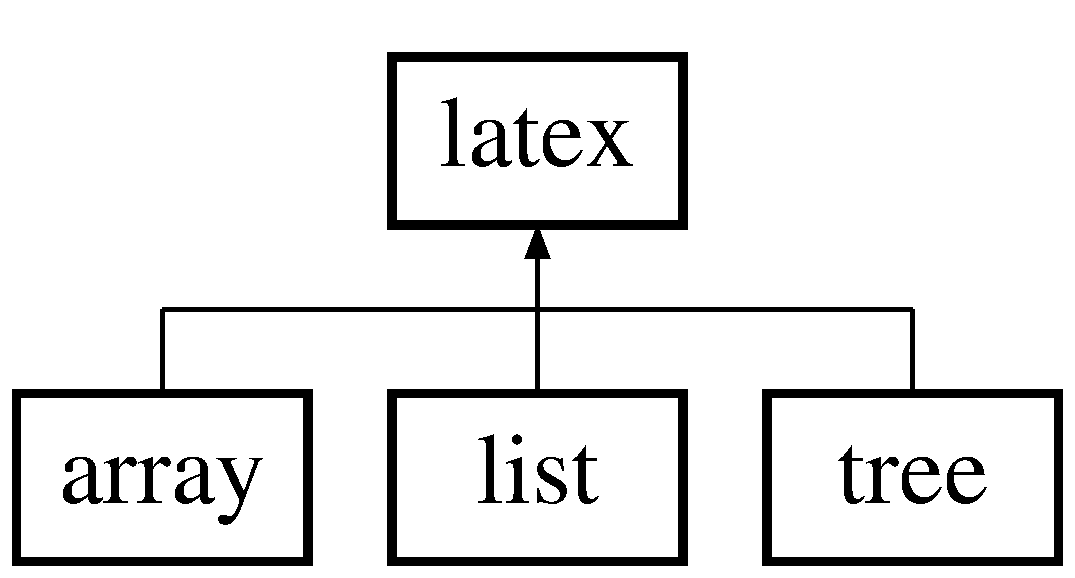
\includegraphics[height=2.000000cm]{classlatex}
\end{center}
\end{figure}
\subsection*{Public Member Functions}
\begin{DoxyCompactItemize}
\item 
virtual string \hyperlink{classlatex_a087cec6e7708a663c6de8fceb5028fa7}{get\-Cadena} ()
\item 
virtual string \hyperlink{classlatex_a2fc1375dd9193d6089e93848f45b577c}{get\-Cadena\-Temp} ()
\item 
\hyperlink{classlatex_aace0b094e1bd77e62505bdaa8c3f6e27}{latex} (void)
\item 
\hyperlink{classlatex_afacb95a7c4d29fa0ecb7c26bd5e383e1}{$\sim$latex} (void)
\end{DoxyCompactItemize}
\subsection*{Protected Attributes}
\begin{DoxyCompactItemize}
\item 
string \hyperlink{classlatex_ad55bec26256e48f114d250bed4a3f35d}{cadena}
\item 
string \hyperlink{classlatex_abe019c68eb9e6be93980f728ee837817}{cadena\-\_\-temp}
\end{DoxyCompactItemize}


\subsection{Constructor \& Destructor Documentation}
\hypertarget{classlatex_aace0b094e1bd77e62505bdaa8c3f6e27}{\index{latex@{latex}!latex@{latex}}
\index{latex@{latex}!latex@{latex}}
\subsubsection[{latex}]{\setlength{\rightskip}{0pt plus 5cm}latex\-::latex (
\begin{DoxyParamCaption}
\item[{void}]{}
\end{DoxyParamCaption}
)}}\label{classlatex_aace0b094e1bd77e62505bdaa8c3f6e27}
\hypertarget{classlatex_afacb95a7c4d29fa0ecb7c26bd5e383e1}{\index{latex@{latex}!$\sim$latex@{$\sim$latex}}
\index{$\sim$latex@{$\sim$latex}!latex@{latex}}
\subsubsection[{$\sim$latex}]{\setlength{\rightskip}{0pt plus 5cm}latex\-::$\sim$latex (
\begin{DoxyParamCaption}
\item[{void}]{}
\end{DoxyParamCaption}
)}}\label{classlatex_afacb95a7c4d29fa0ecb7c26bd5e383e1}


\subsection{Member Function Documentation}
\hypertarget{classlatex_a087cec6e7708a663c6de8fceb5028fa7}{\index{latex@{latex}!get\-Cadena@{get\-Cadena}}
\index{get\-Cadena@{get\-Cadena}!latex@{latex}}
\subsubsection[{get\-Cadena}]{\setlength{\rightskip}{0pt plus 5cm}string latex\-::get\-Cadena (
\begin{DoxyParamCaption}
{}
\end{DoxyParamCaption}
)\hspace{0.3cm}{\ttfamily [virtual]}}}\label{classlatex_a087cec6e7708a663c6de8fceb5028fa7}


Reimplemented in \hyperlink{classarray_ac4088f8ff54a0a4e016ac66b900c976a}{array}, and \hyperlink{classlist_af9c57f43f632e0c885c2393dc375ccf9}{list}.

\hypertarget{classlatex_a2fc1375dd9193d6089e93848f45b577c}{\index{latex@{latex}!get\-Cadena\-Temp@{get\-Cadena\-Temp}}
\index{get\-Cadena\-Temp@{get\-Cadena\-Temp}!latex@{latex}}
\subsubsection[{get\-Cadena\-Temp}]{\setlength{\rightskip}{0pt plus 5cm}string latex\-::get\-Cadena\-Temp (
\begin{DoxyParamCaption}
{}
\end{DoxyParamCaption}
)\hspace{0.3cm}{\ttfamily [virtual]}}}\label{classlatex_a2fc1375dd9193d6089e93848f45b577c}


\subsection{Member Data Documentation}
\hypertarget{classlatex_ad55bec26256e48f114d250bed4a3f35d}{\index{latex@{latex}!cadena@{cadena}}
\index{cadena@{cadena}!latex@{latex}}
\subsubsection[{cadena}]{\setlength{\rightskip}{0pt plus 5cm}string latex\-::cadena\hspace{0.3cm}{\ttfamily [protected]}}}\label{classlatex_ad55bec26256e48f114d250bed4a3f35d}
\hypertarget{classlatex_abe019c68eb9e6be93980f728ee837817}{\index{latex@{latex}!cadena\-\_\-temp@{cadena\-\_\-temp}}
\index{cadena\-\_\-temp@{cadena\-\_\-temp}!latex@{latex}}
\subsubsection[{cadena\-\_\-temp}]{\setlength{\rightskip}{0pt plus 5cm}string latex\-::cadena\-\_\-temp\hspace{0.3cm}{\ttfamily [protected]}}}\label{classlatex_abe019c68eb9e6be93980f728ee837817}


The documentation for this class was generated from the following files\-:\begin{DoxyCompactItemize}
\item 
/home/mtorres/\-Dropbox/\-Universidad/\-Estructuras/\-Proyecto1/\-Fox\-Hound/\-P\-R\-O\-Y\-E\-C\-T\-O/\hyperlink{latex_8h}{latex.\-h}\item 
/home/mtorres/\-Dropbox/\-Universidad/\-Estructuras/\-Proyecto1/\-Fox\-Hound/\-P\-R\-O\-Y\-E\-C\-T\-O/\hyperlink{latex_8cpp}{latex.\-cpp}\end{DoxyCompactItemize}

\hypertarget{classlist}{\section{list Class Reference}
\label{classlist}\index{list@{list}}
}
Inheritance diagram for list\-:\begin{figure}[H]
\begin{center}
\leavevmode
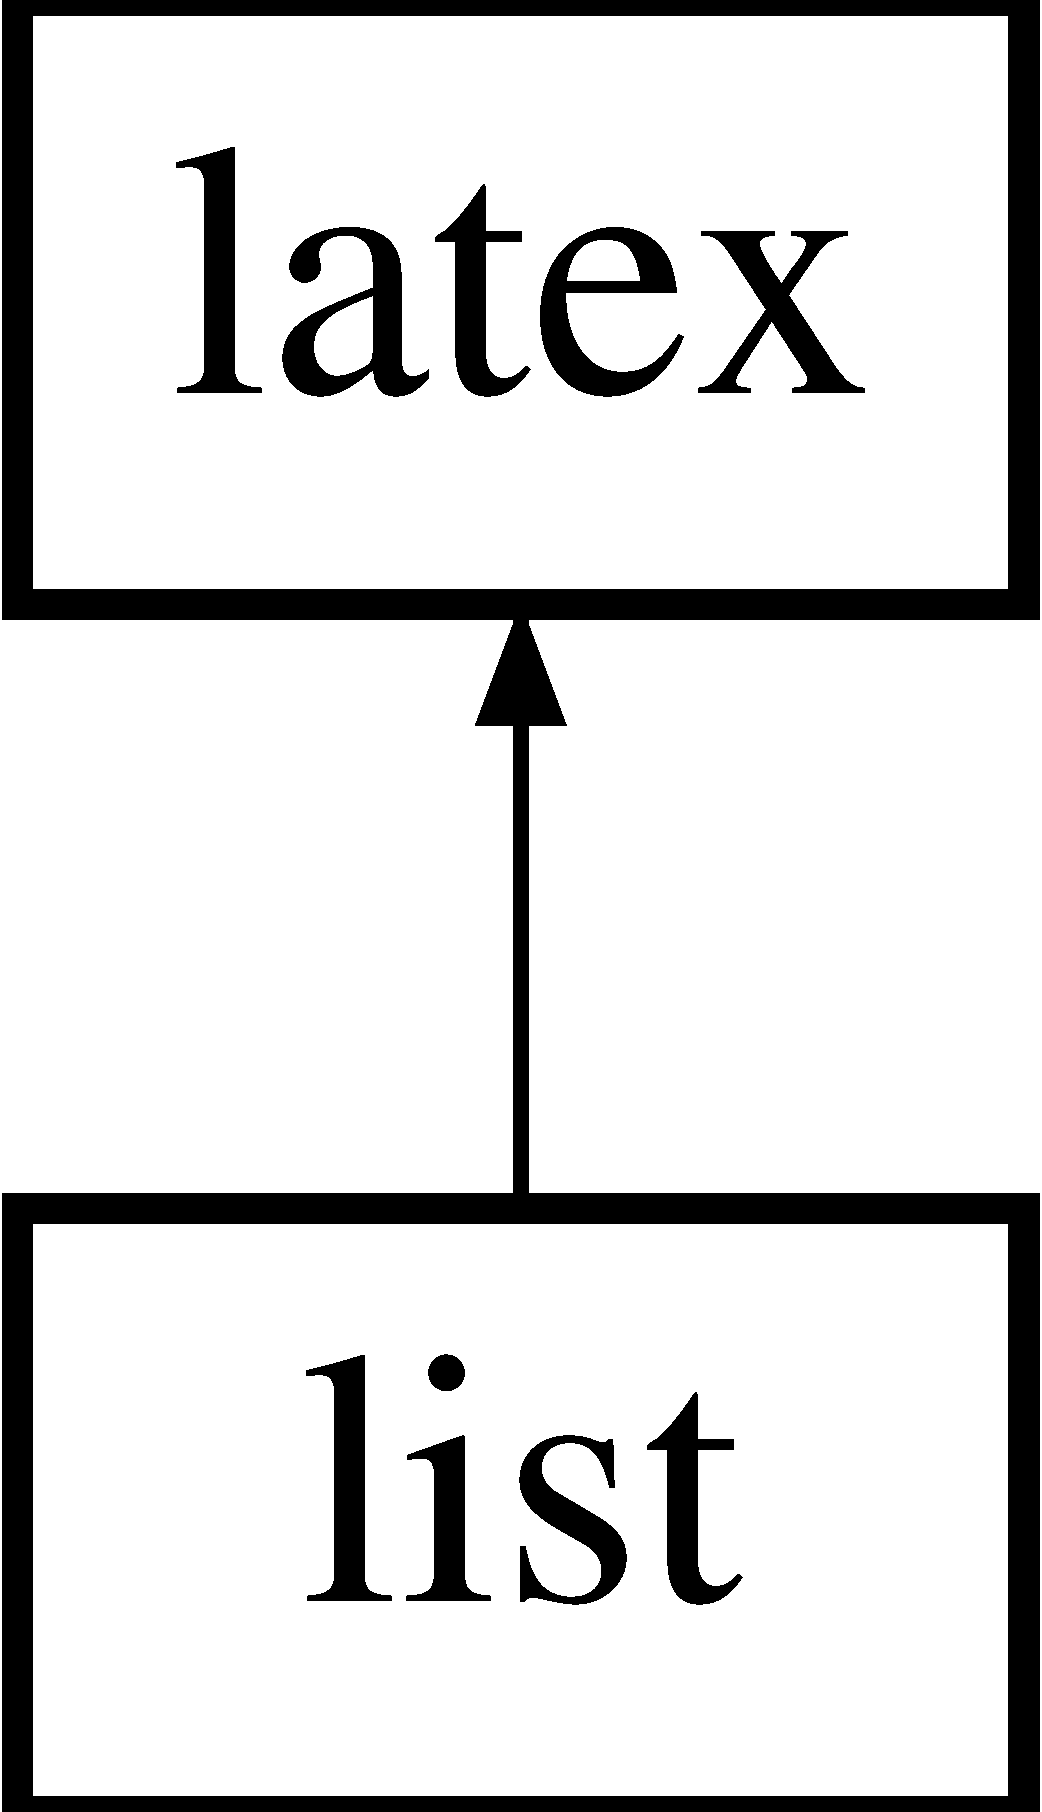
\includegraphics[height=2.000000cm]{classlist}
\end{center}
\end{figure}
\subsection*{Public Member Functions}
\begin{DoxyCompactItemize}
\item 
\hypertarget{classlist_a223ecca7c96ef287c1e647493a32fbf6}{\hyperlink{classlist_a223ecca7c96ef287c1e647493a32fbf6}{list} ()}\label{classlist_a223ecca7c96ef287c1e647493a32fbf6}

\begin{DoxyCompactList}\small\item\em Default constructor. \end{DoxyCompactList}\item 
\hypertarget{classlist_a72eaabb03a048506432f8d167db12524}{\hyperlink{classlist_a72eaabb03a048506432f8d167db12524}{$\sim$list} ()}\label{classlist_a72eaabb03a048506432f8d167db12524}

\begin{DoxyCompactList}\small\item\em Destructor. \end{DoxyCompactList}\item 
\hypertarget{classlist_a7ad1d4788bef2d9ccb1827ed1576eb4e}{bool \hyperlink{classlist_a7ad1d4788bef2d9ccb1827ed1576eb4e}{search} (int v)}\label{classlist_a7ad1d4788bef2d9ccb1827ed1576eb4e}

\begin{DoxyCompactList}\small\item\em Confirms if the value \char`\"{}v\char`\"{} is in the list. \end{DoxyCompactList}\item 
\hypertarget{classlist_a69b02d50b1ec180ca86003eefc427bef}{void \hyperlink{classlist_a69b02d50b1ec180ca86003eefc427bef}{insert\-\_\-at\-\_\-beginning} (int v)}\label{classlist_a69b02d50b1ec180ca86003eefc427bef}

\begin{DoxyCompactList}\small\item\em Inserts a new node with value \char`\"{}v\char`\"{} at beginning of the list. \end{DoxyCompactList}\item 
\hypertarget{classlist_a0aa6499aab860dccd290638f1db18148}{void \hyperlink{classlist_a0aa6499aab860dccd290638f1db18148}{insert\-\_\-at\-\_\-end} (int v)}\label{classlist_a0aa6499aab860dccd290638f1db18148}

\begin{DoxyCompactList}\small\item\em Inserts a new node at end of the list. \end{DoxyCompactList}\item 
\hypertarget{classlist_ac6ae86ceba69b3d9930925e826533fe6}{void \hyperlink{classlist_ac6ae86ceba69b3d9930925e826533fe6}{insert\-\_\-in\-\_\-position} (int v, int pos)}\label{classlist_ac6ae86ceba69b3d9930925e826533fe6}

\begin{DoxyCompactList}\small\item\em Inserts a new node with value \char`\"{}v\char`\"{} in the position \char`\"{}pos\char`\"{} of the list. \end{DoxyCompactList}\item 
\hypertarget{classlist_a9442b8d51977d2e334668c5af309b0a6}{void \hyperlink{classlist_a9442b8d51977d2e334668c5af309b0a6}{delete\-\_\-first\-\_\-node} ()}\label{classlist_a9442b8d51977d2e334668c5af309b0a6}

\begin{DoxyCompactList}\small\item\em Deletes the first node of the list. \end{DoxyCompactList}\item 
\hypertarget{classlist_a940e14191c9749919d81be840b1ce163}{void \hyperlink{classlist_a940e14191c9749919d81be840b1ce163}{delete\-\_\-last\-\_\-node} ()}\label{classlist_a940e14191c9749919d81be840b1ce163}

\begin{DoxyCompactList}\small\item\em Deletes the last node of the list. \end{DoxyCompactList}\item 
\hypertarget{classlist_aad82eb6c4ac56b4d52ceb292aef40232}{void \hyperlink{classlist_aad82eb6c4ac56b4d52ceb292aef40232}{delete\-\_\-in\-\_\-position} (int pos)}\label{classlist_aad82eb6c4ac56b4d52ceb292aef40232}

\begin{DoxyCompactList}\small\item\em Deletes the node in the position \char`\"{}pos\char`\"{}of the list. \end{DoxyCompactList}\item 
\hypertarget{classlist_ab11707b9d85a5c33d0bebf8944c0e857}{void \hyperlink{classlist_ab11707b9d85a5c33d0bebf8944c0e857}{next\-\_\-node} ()}\label{classlist_ab11707b9d85a5c33d0bebf8944c0e857}

\begin{DoxyCompactList}\small\item\em Set the current node in the next node of the list. \end{DoxyCompactList}\item 
\hypertarget{classlist_afb9c1a47eb001496eabd2d3ac37d283d}{void \hyperlink{classlist_afb9c1a47eb001496eabd2d3ac37d283d}{go\-\_\-to\-\_\-first\-\_\-node} ()}\label{classlist_afb9c1a47eb001496eabd2d3ac37d283d}

\begin{DoxyCompactList}\small\item\em Set the current node in the first node of the list. \end{DoxyCompactList}\item 
\hypertarget{classlist_a3d9c0dd74589893d2e8337f6b2fa78ac}{void \hyperlink{classlist_a3d9c0dd74589893d2e8337f6b2fa78ac}{go\-\_\-to\-\_\-last\-\_\-node} ()}\label{classlist_a3d9c0dd74589893d2e8337f6b2fa78ac}

\begin{DoxyCompactList}\small\item\em Set the current node in the last node of the list. \end{DoxyCompactList}\item 
\hypertarget{classlist_af3be16d99b45856c9222dec685628122}{bool \hyperlink{classlist_af3be16d99b45856c9222dec685628122}{get\-\_\-current\-\_\-node} ()}\label{classlist_af3be16d99b45856c9222dec685628122}

\begin{DoxyCompactList}\small\item\em Returns the current node, if this is not N\-U\-L\-L. \end{DoxyCompactList}\item 
\hypertarget{classlist_a4a401135cd9300328664b4295f8bcbb1}{int \hyperlink{classlist_a4a401135cd9300328664b4295f8bcbb1}{current\-\_\-value} ()}\label{classlist_a4a401135cd9300328664b4295f8bcbb1}

\begin{DoxyCompactList}\small\item\em Returns the value of the current node. \end{DoxyCompactList}\item 
\hypertarget{classlist_af9c57f43f632e0c885c2393dc375ccf9}{string {\bfseries get\-Cadena} ()}\label{classlist_af9c57f43f632e0c885c2393dc375ccf9}

\item 
\hypertarget{classlist_a66002d493740d5c50137c428597b4f70}{void \hyperlink{classlist_a66002d493740d5c50137c428597b4f70}{begin\-\_\-tex} (string)}\label{classlist_a66002d493740d5c50137c428597b4f70}

\begin{DoxyCompactList}\small\item\em Writes the headers and required latex libraries and packages on the .tex file. \end{DoxyCompactList}\item 
\hypertarget{classlist_ad0581363cabe43d9524e27321bf19cc0}{void \hyperlink{classlist_ad0581363cabe43d9524e27321bf19cc0}{end\-\_\-tex} ()}\label{classlist_ad0581363cabe43d9524e27321bf19cc0}

\begin{DoxyCompactList}\small\item\em Writes the footers on the .tex file. \end{DoxyCompactList}\item 
\hypertarget{classlist_af38e18a21e1631f6f0e381aefe4262fe}{string \hyperlink{classlist_af38e18a21e1631f6f0e381aefe4262fe}{to\-\_\-string} (int v)}\label{classlist_af38e18a21e1631f6f0e381aefe4262fe}

\begin{DoxyCompactList}\small\item\em Convert an int \char`\"{}v\char`\"{} to string. \end{DoxyCompactList}\end{DoxyCompactItemize}
\subsection*{Public Attributes}
\begin{DoxyCompactItemize}
\item 
\hypertarget{classlist_a3b03adad0c0429bae9493667ff366dc2}{int \hyperlink{classlist_a3b03adad0c0429bae9493667ff366dc2}{size}}\label{classlist_a3b03adad0c0429bae9493667ff366dc2}

\begin{DoxyCompactList}\small\item\em Size of the list. \end{DoxyCompactList}\end{DoxyCompactItemize}
\subsection*{Additional Inherited Members}


The documentation for this class was generated from the following files\-:\begin{DoxyCompactItemize}
\item 
/home/mtorres/\-Dropbox/\-Universidad/\-Estructuras/\-Proyecto1/\-Fox\-Hound/\-P\-R\-O\-Y\-E\-C\-T\-O/list.\-h\item 
/home/mtorres/\-Dropbox/\-Universidad/\-Estructuras/\-Proyecto1/\-Fox\-Hound/\-P\-R\-O\-Y\-E\-C\-T\-O/list.\-cpp\end{DoxyCompactItemize}

\hypertarget{classlist__node}{\section{list\-\_\-node Class Reference}
\label{classlist__node}\index{list\-\_\-node@{list\-\_\-node}}
}
\subsection*{Public Member Functions}
\begin{DoxyCompactItemize}
\item 
\hypertarget{classlist__node_a9b9ef19a716fe4a3e52f5f7b3739caf7}{{\bfseries list\-\_\-node} (int v, \hyperlink{classlist__node}{list\-\_\-node} $\ast$)}\label{classlist__node_a9b9ef19a716fe4a3e52f5f7b3739caf7}

\item 
\hypertarget{classlist__node_a775315187e361ab4dd6a8a3add2ba59c}{void {\bfseries set\-\_\-value} (int)}\label{classlist__node_a775315187e361ab4dd6a8a3add2ba59c}

\item 
\hypertarget{classlist__node_a8248fa0566e951fe9e57e3e110b73f33}{int {\bfseries get\-\_\-value} ()}\label{classlist__node_a8248fa0566e951fe9e57e3e110b73f33}

\item 
\hypertarget{classlist__node_a9808bd1c12f8265d261793b2f60b8b95}{void {\bfseries set\-\_\-next} (\hyperlink{classlist__node}{list\-\_\-node} $\ast$)}\label{classlist__node_a9808bd1c12f8265d261793b2f60b8b95}

\item 
\hypertarget{classlist__node_a8652a8e934c044a5d3e898629173c23f}{\hyperlink{classlist__node}{list\-\_\-node} $\ast$ {\bfseries get\-\_\-next} ()}\label{classlist__node_a8652a8e934c044a5d3e898629173c23f}

\end{DoxyCompactItemize}


The documentation for this class was generated from the following files\-:\begin{DoxyCompactItemize}
\item 
/home/mtorres/\-Dropbox/\-Universidad/\-Estructuras/\-Proyecto1/\-Fox\-Hound/nano/\-Cpp\-\_\-modificable/list\-\_\-node.\-h\item 
/home/mtorres/\-Dropbox/\-Universidad/\-Estructuras/\-Proyecto1/\-Fox\-Hound/nano/\-Cpp\-\_\-modificable/list\-\_\-node.\-cpp\end{DoxyCompactItemize}

\hypertarget{structnode}{\section{node Struct Reference}
\label{structnode}\index{node@{node}}
}


{\ttfamily \#include $<$tree\-\_\-node.\-h$>$}

\subsection*{Public Attributes}
\begin{DoxyCompactItemize}
\item 
int \hyperlink{structnode_a182db137ea0884489bee856c63b33d9a}{key\-\_\-value}
\item 
\hyperlink{structnode}{node} $\ast$ \hyperlink{structnode_a7cbff55ff448f557223f79299056e9b1}{left}
\item 
\hyperlink{structnode}{node} $\ast$ \hyperlink{structnode_abdc86d4c8604c481752953af3235fc47}{right}
\end{DoxyCompactItemize}


\subsection{Member Data Documentation}
\hypertarget{structnode_a182db137ea0884489bee856c63b33d9a}{\index{node@{node}!key\-\_\-value@{key\-\_\-value}}
\index{key\-\_\-value@{key\-\_\-value}!node@{node}}
\subsubsection[{key\-\_\-value}]{\setlength{\rightskip}{0pt plus 5cm}int node\-::key\-\_\-value}}\label{structnode_a182db137ea0884489bee856c63b33d9a}
\hypertarget{structnode_a7cbff55ff448f557223f79299056e9b1}{\index{node@{node}!left@{left}}
\index{left@{left}!node@{node}}
\subsubsection[{left}]{\setlength{\rightskip}{0pt plus 5cm}{\bf node}$\ast$ node\-::left}}\label{structnode_a7cbff55ff448f557223f79299056e9b1}
\hypertarget{structnode_abdc86d4c8604c481752953af3235fc47}{\index{node@{node}!right@{right}}
\index{right@{right}!node@{node}}
\subsubsection[{right}]{\setlength{\rightskip}{0pt plus 5cm}{\bf node}$\ast$ node\-::right}}\label{structnode_abdc86d4c8604c481752953af3235fc47}


The documentation for this struct was generated from the following file\-:\begin{DoxyCompactItemize}
\item 
/home/mtorres/\-Dropbox/\-Universidad/\-Estructuras/\-Proyecto1/\-Fox\-Hound/\-P\-R\-O\-Y\-E\-C\-T\-O/\hyperlink{tree__node_8h}{tree\-\_\-node.\-h}\end{DoxyCompactItemize}

\hypertarget{classtree}{\section{tree Class Reference}
\label{classtree}\index{tree@{tree}}
}


{\ttfamily \#include $<$tree.\-h$>$}

Inheritance diagram for tree\-:\begin{figure}[H]
\begin{center}
\leavevmode
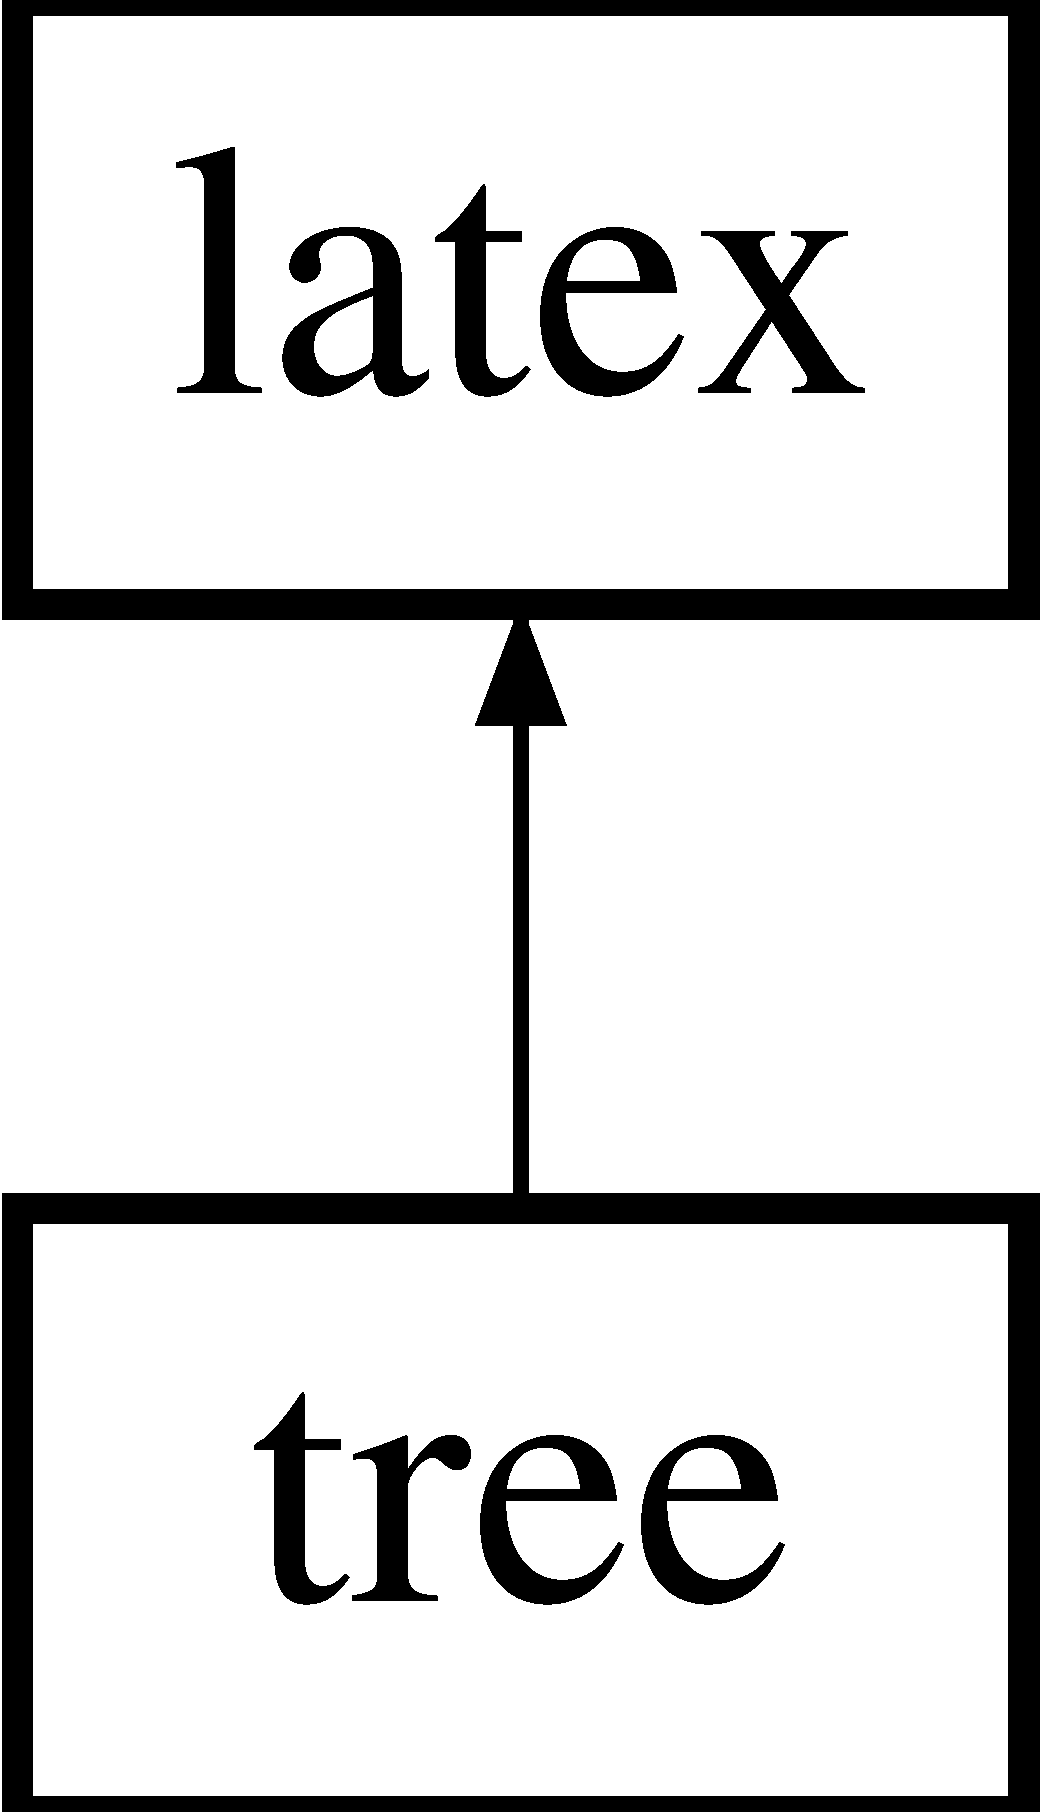
\includegraphics[height=2.000000cm]{classtree}
\end{center}
\end{figure}
\subsection*{Public Member Functions}
\begin{DoxyCompactItemize}
\item 
\hyperlink{classtree_a9f2a566ac2710fafc31232456780e82d}{tree} ()
\begin{DoxyCompactList}\small\item\em Default constructor. \end{DoxyCompactList}\item 
\hyperlink{classtree_a05f3faa3c9a8f6fed237e2d0f6172244}{$\sim$tree} ()
\begin{DoxyCompactList}\small\item\em Destructor. \end{DoxyCompactList}\item 
void \hyperlink{classtree_acbfbccebf3d8482cb6a1a878ab99491f}{insert\-\_\-root} (int key)
\begin{DoxyCompactList}\small\item\em Inserts the root node of the tree, initially its leaves are pointing to N\-U\-L\-L. \end{DoxyCompactList}\item 
void \hyperlink{classtree_a523172b004801388b1e6920d6d984347}{destroy\-\_\-tree} ()
\begin{DoxyCompactList}\small\item\em Destroy each leaf if is not points to N\-U\-L\-L. \end{DoxyCompactList}\item 
void \hyperlink{classtree_adebed7ad744b6db3354bfdc9a6713143}{insert\-\_\-child} (int key, \hyperlink{structnode}{node} $\ast$leaf)
\begin{DoxyCompactList}\small\item\em Inserts a leaf with value \char`\"{}key\char`\"{} in the node \char`\"{}leaf\char`\"{}. \end{DoxyCompactList}\item 
\hyperlink{structnode}{node} $\ast$ \hyperlink{classtree_a9a4e341c78d3559e5f6e3b0060530f05}{search} (int key)
\begin{DoxyCompactList}\small\item\em Returns the node with the key\-\_\-value \char`\"{}key\char`\"{}. \end{DoxyCompactList}\item 
void \hyperlink{classtree_a86bf515529211e7f7d1f18892bf6fff5}{finish\-\_\-tree} ()
\begin{DoxyCompactList}\small\item\em Draws the tree on the .tex file. \end{DoxyCompactList}\item 
\hyperlink{structnode}{node} $\ast$ \hyperlink{classtree_a4fe0fb0307507a56395a377d2166d4d2}{return\-\_\-root} ()
\begin{DoxyCompactList}\small\item\em Returns the root of the tree. \end{DoxyCompactList}\end{DoxyCompactItemize}
\subsection*{Additional Inherited Members}


\subsection{Constructor \& Destructor Documentation}
\hypertarget{classtree_a9f2a566ac2710fafc31232456780e82d}{\index{tree@{tree}!tree@{tree}}
\index{tree@{tree}!tree@{tree}}
\subsubsection[{tree}]{\setlength{\rightskip}{0pt plus 5cm}tree\-::tree (
\begin{DoxyParamCaption}
{}
\end{DoxyParamCaption}
)}}\label{classtree_a9f2a566ac2710fafc31232456780e82d}


Default constructor. 

\hypertarget{classtree_a05f3faa3c9a8f6fed237e2d0f6172244}{\index{tree@{tree}!$\sim$tree@{$\sim$tree}}
\index{$\sim$tree@{$\sim$tree}!tree@{tree}}
\subsubsection[{$\sim$tree}]{\setlength{\rightskip}{0pt plus 5cm}tree\-::$\sim$tree (
\begin{DoxyParamCaption}
{}
\end{DoxyParamCaption}
)}}\label{classtree_a05f3faa3c9a8f6fed237e2d0f6172244}


Destructor. 



\subsection{Member Function Documentation}
\hypertarget{classtree_a523172b004801388b1e6920d6d984347}{\index{tree@{tree}!destroy\-\_\-tree@{destroy\-\_\-tree}}
\index{destroy\-\_\-tree@{destroy\-\_\-tree}!tree@{tree}}
\subsubsection[{destroy\-\_\-tree}]{\setlength{\rightskip}{0pt plus 5cm}void tree\-::destroy\-\_\-tree (
\begin{DoxyParamCaption}
{}
\end{DoxyParamCaption}
)}}\label{classtree_a523172b004801388b1e6920d6d984347}


Destroy each leaf if is not points to N\-U\-L\-L. 

\hypertarget{classtree_a86bf515529211e7f7d1f18892bf6fff5}{\index{tree@{tree}!finish\-\_\-tree@{finish\-\_\-tree}}
\index{finish\-\_\-tree@{finish\-\_\-tree}!tree@{tree}}
\subsubsection[{finish\-\_\-tree}]{\setlength{\rightskip}{0pt plus 5cm}void tree\-::finish\-\_\-tree (
\begin{DoxyParamCaption}
{}
\end{DoxyParamCaption}
)}}\label{classtree_a86bf515529211e7f7d1f18892bf6fff5}


Draws the tree on the .tex file. 

\hypertarget{classtree_adebed7ad744b6db3354bfdc9a6713143}{\index{tree@{tree}!insert\-\_\-child@{insert\-\_\-child}}
\index{insert\-\_\-child@{insert\-\_\-child}!tree@{tree}}
\subsubsection[{insert\-\_\-child}]{\setlength{\rightskip}{0pt plus 5cm}void tree\-::insert\-\_\-child (
\begin{DoxyParamCaption}
\item[{int}]{key, }
\item[{{\bf node} $\ast$}]{leaf}
\end{DoxyParamCaption}
)}}\label{classtree_adebed7ad744b6db3354bfdc9a6713143}


Inserts a leaf with value \char`\"{}key\char`\"{} in the node \char`\"{}leaf\char`\"{}. 

\hypertarget{classtree_acbfbccebf3d8482cb6a1a878ab99491f}{\index{tree@{tree}!insert\-\_\-root@{insert\-\_\-root}}
\index{insert\-\_\-root@{insert\-\_\-root}!tree@{tree}}
\subsubsection[{insert\-\_\-root}]{\setlength{\rightskip}{0pt plus 5cm}void tree\-::insert\-\_\-root (
\begin{DoxyParamCaption}
\item[{int}]{key}
\end{DoxyParamCaption}
)}}\label{classtree_acbfbccebf3d8482cb6a1a878ab99491f}


Inserts the root node of the tree, initially its leaves are pointing to N\-U\-L\-L. 

\hypertarget{classtree_a4fe0fb0307507a56395a377d2166d4d2}{\index{tree@{tree}!return\-\_\-root@{return\-\_\-root}}
\index{return\-\_\-root@{return\-\_\-root}!tree@{tree}}
\subsubsection[{return\-\_\-root}]{\setlength{\rightskip}{0pt plus 5cm}{\bf node} $\ast$ tree\-::return\-\_\-root (
\begin{DoxyParamCaption}
{}
\end{DoxyParamCaption}
)}}\label{classtree_a4fe0fb0307507a56395a377d2166d4d2}


Returns the root of the tree. 

\hypertarget{classtree_a9a4e341c78d3559e5f6e3b0060530f05}{\index{tree@{tree}!search@{search}}
\index{search@{search}!tree@{tree}}
\subsubsection[{search}]{\setlength{\rightskip}{0pt plus 5cm}{\bf node} $\ast$ tree\-::search (
\begin{DoxyParamCaption}
\item[{int}]{key}
\end{DoxyParamCaption}
)}}\label{classtree_a9a4e341c78d3559e5f6e3b0060530f05}


Returns the node with the key\-\_\-value \char`\"{}key\char`\"{}. 



The documentation for this class was generated from the following files\-:\begin{DoxyCompactItemize}
\item 
/home/mtorres/\-Dropbox/\-Universidad/\-Estructuras/\-Proyecto1/\-Fox\-Hound/\-P\-R\-O\-Y\-E\-C\-T\-O/\hyperlink{tree_8h}{tree.\-h}\item 
/home/mtorres/\-Dropbox/\-Universidad/\-Estructuras/\-Proyecto1/\-Fox\-Hound/\-P\-R\-O\-Y\-E\-C\-T\-O/\hyperlink{tree_8cpp}{tree.\-cpp}\end{DoxyCompactItemize}

\chapter{File Documentation}
\hypertarget{array_8cpp}{\section{/home/mtorres/\-Dropbox/\-Universidad/\-Estructuras/\-Proyecto1/\-Fox\-Hound/src/array.cpp File Reference}
\label{array_8cpp}\index{/home/mtorres/\-Dropbox/\-Universidad/\-Estructuras/\-Proyecto1/\-Fox\-Hound/src/array.\-cpp@{/home/mtorres/\-Dropbox/\-Universidad/\-Estructuras/\-Proyecto1/\-Fox\-Hound/src/array.\-cpp}}
}
{\ttfamily \#include \char`\"{}array.\-h\char`\"{}}\\*
{\ttfamily \#include $<$iostream$>$}\\*
{\ttfamily \#include $<$sstream$>$}\\*

\hypertarget{array_8h}{\section{/home/mtorres/\-Dropbox/\-Universidad/\-Estructuras/\-Proyecto1/\-Fox\-Hound/src/array.h File Reference}
\label{array_8h}\index{/home/mtorres/\-Dropbox/\-Universidad/\-Estructuras/\-Proyecto1/\-Fox\-Hound/src/array.\-h@{/home/mtorres/\-Dropbox/\-Universidad/\-Estructuras/\-Proyecto1/\-Fox\-Hound/src/array.\-h}}
}
{\ttfamily \#include \char`\"{}latex.\-h\char`\"{}}\\*
\subsection*{Classes}
\begin{DoxyCompactItemize}
\item 
class \hyperlink{classarray}{array}
\end{DoxyCompactItemize}

\hypertarget{mainpage_8dox}{\section{/home/mtorres/\-Dropbox/\-Universidad/\-Estructuras/\-Proyecto1/\-Fox\-Hound/src/doc\-\_\-files/mainpage.dox File Reference}
\label{mainpage_8dox}\index{/home/mtorres/\-Dropbox/\-Universidad/\-Estructuras/\-Proyecto1/\-Fox\-Hound/src/doc\-\_\-files/mainpage.\-dox@{/home/mtorres/\-Dropbox/\-Universidad/\-Estructuras/\-Proyecto1/\-Fox\-Hound/src/doc\-\_\-files/mainpage.\-dox}}
}

\hypertarget{latex_8cpp}{\section{/home/mtorres/\-Dropbox/\-Universidad/\-Estructuras/\-Proyecto1/\-Fox\-Hound/\-P\-R\-O\-Y\-E\-C\-T\-O/latex.cpp File Reference}
\label{latex_8cpp}\index{/home/mtorres/\-Dropbox/\-Universidad/\-Estructuras/\-Proyecto1/\-Fox\-Hound/\-P\-R\-O\-Y\-E\-C\-T\-O/latex.\-cpp@{/home/mtorres/\-Dropbox/\-Universidad/\-Estructuras/\-Proyecto1/\-Fox\-Hound/\-P\-R\-O\-Y\-E\-C\-T\-O/latex.\-cpp}}
}
{\ttfamily \#include \char`\"{}latex.\-h\char`\"{}}\\*

\hypertarget{latex_8h}{\section{/home/mtorres/\-Dropbox/\-Universidad/\-Estructuras/\-Proyecto1/\-Fox\-Hound/src/latex.h File Reference}
\label{latex_8h}\index{/home/mtorres/\-Dropbox/\-Universidad/\-Estructuras/\-Proyecto1/\-Fox\-Hound/src/latex.\-h@{/home/mtorres/\-Dropbox/\-Universidad/\-Estructuras/\-Proyecto1/\-Fox\-Hound/src/latex.\-h}}
}
{\ttfamily \#include $<$string$>$}\\*
\subsection*{Classes}
\begin{DoxyCompactItemize}
\item 
class \hyperlink{classlatex}{latex}
\end{DoxyCompactItemize}
\subsection*{Macros}
\begin{DoxyCompactItemize}
\item 
\#define \hyperlink{latex_8h_a351a9532b84f9a97732cad49a8716a92}{L\-A\-T\-E\-X}
\end{DoxyCompactItemize}


\subsection{Macro Definition Documentation}
\hypertarget{latex_8h_a351a9532b84f9a97732cad49a8716a92}{\index{latex.\-h@{latex.\-h}!L\-A\-T\-E\-X@{L\-A\-T\-E\-X}}
\index{L\-A\-T\-E\-X@{L\-A\-T\-E\-X}!latex.h@{latex.\-h}}
\subsubsection[{L\-A\-T\-E\-X}]{\setlength{\rightskip}{0pt plus 5cm}\#define L\-A\-T\-E\-X}}\label{latex_8h_a351a9532b84f9a97732cad49a8716a92}

\hypertarget{list_8cpp}{\section{/home/mtorres/\-Dropbox/\-Universidad/\-Estructuras/\-Proyecto1/\-Fox\-Hound/src/list.cpp File Reference}
\label{list_8cpp}\index{/home/mtorres/\-Dropbox/\-Universidad/\-Estructuras/\-Proyecto1/\-Fox\-Hound/src/list.\-cpp@{/home/mtorres/\-Dropbox/\-Universidad/\-Estructuras/\-Proyecto1/\-Fox\-Hound/src/list.\-cpp}}
}
{\ttfamily \#include \char`\"{}list.\-h\char`\"{}}\\*
{\ttfamily \#include $<$iostream$>$}\\*
{\ttfamily \#include $<$sstream$>$}\\*

\hypertarget{list_8h}{\section{/home/mtorres/\-Dropbox/\-Universidad/\-Estructuras/\-Proyecto1/\-Fox\-Hound/\-P\-R\-O\-Y\-E\-C\-T\-O/list.h File Reference}
\label{list_8h}\index{/home/mtorres/\-Dropbox/\-Universidad/\-Estructuras/\-Proyecto1/\-Fox\-Hound/\-P\-R\-O\-Y\-E\-C\-T\-O/list.\-h@{/home/mtorres/\-Dropbox/\-Universidad/\-Estructuras/\-Proyecto1/\-Fox\-Hound/\-P\-R\-O\-Y\-E\-C\-T\-O/list.\-h}}
}
{\ttfamily \#include \char`\"{}latex.\-h\char`\"{}}\\*
{\ttfamily \#include \char`\"{}list\-\_\-node.\-h\char`\"{}}\\*
\subsection*{Classes}
\begin{DoxyCompactItemize}
\item 
class \hyperlink{classlist}{list}
\end{DoxyCompactItemize}

\hypertarget{list__node_8cpp}{\section{/home/mtorres/\-Dropbox/\-Universidad/\-Estructuras/\-Proyecto1/\-Fox\-Hound/src/list\-\_\-node.cpp File Reference}
\label{list__node_8cpp}\index{/home/mtorres/\-Dropbox/\-Universidad/\-Estructuras/\-Proyecto1/\-Fox\-Hound/src/list\-\_\-node.\-cpp@{/home/mtorres/\-Dropbox/\-Universidad/\-Estructuras/\-Proyecto1/\-Fox\-Hound/src/list\-\_\-node.\-cpp}}
}
{\ttfamily \#include \char`\"{}list\-\_\-node.\-h\char`\"{}}\\*
{\ttfamily \#include $<$iostream$>$}\\*

\hypertarget{list__node_8h}{\section{/home/mtorres/\-Dropbox/\-Universidad/\-Estructuras/\-Proyecto1/\-Fox\-Hound/src/list\-\_\-node.h File Reference}
\label{list__node_8h}\index{/home/mtorres/\-Dropbox/\-Universidad/\-Estructuras/\-Proyecto1/\-Fox\-Hound/src/list\-\_\-node.\-h@{/home/mtorres/\-Dropbox/\-Universidad/\-Estructuras/\-Proyecto1/\-Fox\-Hound/src/list\-\_\-node.\-h}}
}
\subsection*{Classes}
\begin{DoxyCompactItemize}
\item 
class \hyperlink{classlist__node}{list\-\_\-node}
\end{DoxyCompactItemize}

\hypertarget{main_8cpp}{\section{/home/mtorres/\-Dropbox/\-Universidad/\-Estructuras/\-Proyecto1/\-Fox\-Hound/src/main.cpp File Reference}
\label{main_8cpp}\index{/home/mtorres/\-Dropbox/\-Universidad/\-Estructuras/\-Proyecto1/\-Fox\-Hound/src/main.\-cpp@{/home/mtorres/\-Dropbox/\-Universidad/\-Estructuras/\-Proyecto1/\-Fox\-Hound/src/main.\-cpp}}
}
{\ttfamily \#include $<$iostream$>$}\\*
{\ttfamily \#include $<$sstream$>$}\\*
{\ttfamily \#include $<$string$>$}\\*
{\ttfamily \#include \char`\"{}array.\-h\char`\"{}}\\*
{\ttfamily \#include \char`\"{}list.\-h\char`\"{}}\\*
{\ttfamily \#include \char`\"{}tree.\-h\char`\"{}}\\*
{\ttfamily \#include \char`\"{}to\-\_\-tex.\-h\char`\"{}}\\*
\subsection*{Functions}
\begin{DoxyCompactItemize}
\item 
int \hyperlink{main_8cpp_ae66f6b31b5ad750f1fe042a706a4e3d4}{main} ()
\end{DoxyCompactItemize}


\subsection{Function Documentation}
\hypertarget{main_8cpp_ae66f6b31b5ad750f1fe042a706a4e3d4}{\index{main.\-cpp@{main.\-cpp}!main@{main}}
\index{main@{main}!main.cpp@{main.\-cpp}}
\subsubsection[{main}]{\setlength{\rightskip}{0pt plus 5cm}int main (
\begin{DoxyParamCaption}
{}
\end{DoxyParamCaption}
)}}\label{main_8cpp_ae66f6b31b5ad750f1fe042a706a4e3d4}

\hypertarget{to__tex_8cpp}{\section{/home/mtorres/\-Dropbox/\-Universidad/\-Estructuras/\-Proyecto1/\-Fox\-Hound/src/to\-\_\-tex.cpp File Reference}
\label{to__tex_8cpp}\index{/home/mtorres/\-Dropbox/\-Universidad/\-Estructuras/\-Proyecto1/\-Fox\-Hound/src/to\-\_\-tex.\-cpp@{/home/mtorres/\-Dropbox/\-Universidad/\-Estructuras/\-Proyecto1/\-Fox\-Hound/src/to\-\_\-tex.\-cpp}}
}
{\ttfamily \#include \char`\"{}to\-\_\-tex.\-h\char`\"{}}\\*
{\ttfamily \#include $<$string$>$}\\*
{\ttfamily \#include $<$stdlib.\-h$>$}\\*
\subsection*{Functions}
\begin{DoxyCompactItemize}
\item 
void \hyperlink{to__tex_8cpp_a2388a2435840a9bcd64744a8010065e8}{create\-\_\-tex} (string file\-\_\-name, string cadena)
\end{DoxyCompactItemize}


\subsection{Function Documentation}
\hypertarget{to__tex_8cpp_a2388a2435840a9bcd64744a8010065e8}{\index{to\-\_\-tex.\-cpp@{to\-\_\-tex.\-cpp}!create\-\_\-tex@{create\-\_\-tex}}
\index{create\-\_\-tex@{create\-\_\-tex}!to_tex.cpp@{to\-\_\-tex.\-cpp}}
\subsubsection[{create\-\_\-tex}]{\setlength{\rightskip}{0pt plus 5cm}void create\-\_\-tex (
\begin{DoxyParamCaption}
\item[{string}]{file\-\_\-name, }
\item[{string}]{cadena}
\end{DoxyParamCaption}
)}}\label{to__tex_8cpp_a2388a2435840a9bcd64744a8010065e8}

\hypertarget{to__tex_8h}{\section{/home/mtorres/\-Dropbox/\-Universidad/\-Estructuras/\-Proyecto1/\-Fox\-Hound/\-P\-R\-O\-Y\-E\-C\-T\-O/to\-\_\-tex.h File Reference}
\label{to__tex_8h}\index{/home/mtorres/\-Dropbox/\-Universidad/\-Estructuras/\-Proyecto1/\-Fox\-Hound/\-P\-R\-O\-Y\-E\-C\-T\-O/to\-\_\-tex.\-h@{/home/mtorres/\-Dropbox/\-Universidad/\-Estructuras/\-Proyecto1/\-Fox\-Hound/\-P\-R\-O\-Y\-E\-C\-T\-O/to\-\_\-tex.\-h}}
}
{\ttfamily \#include $<$iostream$>$}\\*
{\ttfamily \#include $<$sstream$>$}\\*
{\ttfamily \#include $<$fstream$>$}\\*
{\ttfamily \#include $<$stdio.\-h$>$}\\*
{\ttfamily \#include $<$string$>$}\\*
\subsection*{Functions}
\begin{DoxyCompactItemize}
\item 
void \hyperlink{to__tex_8h_a33c6a7daae498712c94a59d37b3fc2d5}{create\-\_\-tex} (string, string)
\end{DoxyCompactItemize}


\subsection{Function Documentation}
\hypertarget{to__tex_8h_a33c6a7daae498712c94a59d37b3fc2d5}{\index{to\-\_\-tex.\-h@{to\-\_\-tex.\-h}!create\-\_\-tex@{create\-\_\-tex}}
\index{create\-\_\-tex@{create\-\_\-tex}!to_tex.h@{to\-\_\-tex.\-h}}
\subsubsection[{create\-\_\-tex}]{\setlength{\rightskip}{0pt plus 5cm}void create\-\_\-tex (
\begin{DoxyParamCaption}
\item[{string}]{, }
\item[{string}]{}
\end{DoxyParamCaption}
)}}\label{to__tex_8h_a33c6a7daae498712c94a59d37b3fc2d5}

\hypertarget{tree_8cpp}{\section{/home/mtorres/\-Dropbox/\-Universidad/\-Estructuras/\-Proyecto1/\-Fox\-Hound/src/tree.cpp File Reference}
\label{tree_8cpp}\index{/home/mtorres/\-Dropbox/\-Universidad/\-Estructuras/\-Proyecto1/\-Fox\-Hound/src/tree.\-cpp@{/home/mtorres/\-Dropbox/\-Universidad/\-Estructuras/\-Proyecto1/\-Fox\-Hound/src/tree.\-cpp}}
}
{\ttfamily \#include \char`\"{}tree.\-h\char`\"{}}\\*
{\ttfamily \#include $<$iostream$>$}\\*
\subsection*{Variables}
\begin{DoxyCompactItemize}
\item 
int \hyperlink{tree_8cpp_a2c6a3fb7cddd9bd7254692264962b5b3}{contador} =0
\item 
int \hyperlink{tree_8cpp_a8eef4dec947b0a63b5ea6771b51a0484}{contador2} =0
\item 
int \hyperlink{tree_8cpp_ac2bb0fc1fabbeabad94c3b726bd708bc}{variable} =0
\end{DoxyCompactItemize}


\subsection{Variable Documentation}
\hypertarget{tree_8cpp_a2c6a3fb7cddd9bd7254692264962b5b3}{\index{tree.\-cpp@{tree.\-cpp}!contador@{contador}}
\index{contador@{contador}!tree.cpp@{tree.\-cpp}}
\subsubsection[{contador}]{\setlength{\rightskip}{0pt plus 5cm}int contador =0}}\label{tree_8cpp_a2c6a3fb7cddd9bd7254692264962b5b3}
\hypertarget{tree_8cpp_a8eef4dec947b0a63b5ea6771b51a0484}{\index{tree.\-cpp@{tree.\-cpp}!contador2@{contador2}}
\index{contador2@{contador2}!tree.cpp@{tree.\-cpp}}
\subsubsection[{contador2}]{\setlength{\rightskip}{0pt plus 5cm}int contador2 =0}}\label{tree_8cpp_a8eef4dec947b0a63b5ea6771b51a0484}
\hypertarget{tree_8cpp_ac2bb0fc1fabbeabad94c3b726bd708bc}{\index{tree.\-cpp@{tree.\-cpp}!variable@{variable}}
\index{variable@{variable}!tree.cpp@{tree.\-cpp}}
\subsubsection[{variable}]{\setlength{\rightskip}{0pt plus 5cm}int variable =0}}\label{tree_8cpp_ac2bb0fc1fabbeabad94c3b726bd708bc}

\hypertarget{tree_8h}{\section{/home/mtorres/\-Dropbox/\-Universidad/\-Estructuras/\-Proyecto1/\-Fox\-Hound/\-P\-R\-O\-Y\-E\-C\-T\-O/tree.h File Reference}
\label{tree_8h}\index{/home/mtorres/\-Dropbox/\-Universidad/\-Estructuras/\-Proyecto1/\-Fox\-Hound/\-P\-R\-O\-Y\-E\-C\-T\-O/tree.\-h@{/home/mtorres/\-Dropbox/\-Universidad/\-Estructuras/\-Proyecto1/\-Fox\-Hound/\-P\-R\-O\-Y\-E\-C\-T\-O/tree.\-h}}
}
{\ttfamily \#include \char`\"{}tree\-\_\-node.\-h\char`\"{}}\\*
{\ttfamily \#include \char`\"{}latex.\-h\char`\"{}}\\*
{\ttfamily \#include $<$string$>$}\\*
{\ttfamily \#include $<$sstream$>$}\\*
{\ttfamily \#include $<$algorithm$>$}\\*
{\ttfamily \#include $<$fstream$>$}\\*
\subsection*{Classes}
\begin{DoxyCompactItemize}
\item 
class \hyperlink{classtree}{tree}
\end{DoxyCompactItemize}

\hypertarget{tree__node_8h}{\section{/home/mtorres/\-Dropbox/\-Universidad/\-Estructuras/\-Proyecto1/\-Fox\-Hound/src/tree\-\_\-node.h File Reference}
\label{tree__node_8h}\index{/home/mtorres/\-Dropbox/\-Universidad/\-Estructuras/\-Proyecto1/\-Fox\-Hound/src/tree\-\_\-node.\-h@{/home/mtorres/\-Dropbox/\-Universidad/\-Estructuras/\-Proyecto1/\-Fox\-Hound/src/tree\-\_\-node.\-h}}
}
{\ttfamily \#include $<$iostream$>$}\\*
\subsection*{Classes}
\begin{DoxyCompactItemize}
\item 
struct \hyperlink{structnode}{node}
\end{DoxyCompactItemize}

%--- End generated contents ---

% Index
\newpage
\phantomsection
\addcontentsline{toc}{part}{Index}
\printindex

\end{document}
